%--------------------------------------------------------------------------------
%\documentclass{article}

\documentclass[12pt]{article}
\usepackage[T1]{fontenc} 
\usepackage[bf]{caption}
\usepackage{hyperref}
\usepackage[all]{hypcap}
\usepackage[utf8]{inputenc}
\usepackage{graphicx}
\usepackage[czech, english]{babel}
\selectlanguage{czech}
\usepackage{subfig}                % \subfloat
\usepackage{color}
\usepackage{url}
\inputencoding{utf8}
%\usepackage[bf]{caption2}
\usepackage{hyperref}
\usepackage[all]{hypcap}
\hypersetup{colorlinks=false, linkbordercolor=1 1 1, citebordercolor=1 1 1}
\usepackage[right]{lineno}
\renewcommand\linenumberfont{\normalfont\tiny\color{blue}}

\title{FIT VUT, Počítačové Vidění\\Comic Sans OCR}
\author{Miloslav Číž <xcizmi00>, Daniel Žůrek <xzurek12>}
\date{\today}

%--------------------------------------------------------------------------------

\begin{document}
\selectlanguage{czech}
\maketitle

\pagebreak[4]

\section{Zadání a cíle}

Měli jsme implementovat OCR systém pomocí knihovny OpenCV, přičemž jsme mohli
předpokládat dobrou kvalitu skenovaného textu (málo šumu, dobré zarovnání, bez geometrickcých
deformací apod.). Mohli jsme se rovněž omezit na jeden font. Zadání jsme si upřesnili takto:

\begin{itemize}
  \item OCR systém pomocí C++ a~OpenCV, nabízející několik klasifikátorů
  \item Rozpoznávány budou jen znaky anglické abecedy a~některé speciální znaky:
  \begin{itemize}
    \item malá písmena: "abcdefghijklmnopqrstuvwxyz"
    \item velká písmena: "ABCDEFGHIJKLMNOPQRSTUVWXYZ"
    \item číslice: "0123456789"
    \item speciální znaky: ".,-?"
  \end{itemize}
  \item Rozpoznáván bude jen font Comic Sans.
\end{itemize}

Cílem bylo vyzkoušet a~porovnat různé metody používané pro přepis textu. Cílem nebylo udělat
obecný, velmi robustní nebo optimalizovaný OCR systém.

%%%%%%%%%%%%%%%%%%%%%%%%%%%%%%%%%%%%%%%%%%%%%%%%%%%%%%%%%%%%%%%%%%%%%%%%%%%%%%%%%%%%%%%%

\section{Řešení}

Systém se dá rozdělit na dvě části: segmentace a~klasifikace. Museli jsme také vytvořit
dataset pro trénování klasifikátorů a~pro testování.

Práce v~týmu byla rozdělena takto:

\begin{itemize}
  \item Miloslav Číž - dataset, segmentace, MLP, rastr. klas., ukládání do souborů, testování, dokumentace
  \item David Žůrek - KNN, SVM
\end{itemize}

\subsection{Dataset}
\label{sec:dataset}

Pro účely testování jsme napsali sedm A4 stran textu v~programu LibreOffice Writer fontem Comic Sans. Volili jsme
různé velikosti fontu (nejčastěji 12 bodů), řádkování a~různá zarovnání. Texty byly většinou zkopírovány z~anglických internetových
stránek jako Wikipedia nebo Reddit. Stránky jsme následně vytiskli a~naskenovali v~rozlišení $2480 \times 3507$ pixelů.
Dále jsme vytvořili zmenšené a~zašuměné verze stránek. Rovněž jsme z~LibreOffice dokumentů extrahovali čistý text
pro pozdější testování kvality přepisu.

Dataset jednotlivých znaků jsme po implementaci segmentace vytvořili segmentací naskenovaných stránek a~ruční
anotací získaných výřezů. Získali jsme cca 3000 anotovaných vzorků. Dataset je dostupný spolu s~kódem a~skenovanými stránkami
na serveru GitHub. \footnote{https://github.com/drummyfish/Comic-Sans-OCR} Pomocí Python skriptu jsme
vytvořili průměrný obraz každého vzorku pro případné potřeby klasifikátorů.

\begin{figure}[htb]
  \centering
  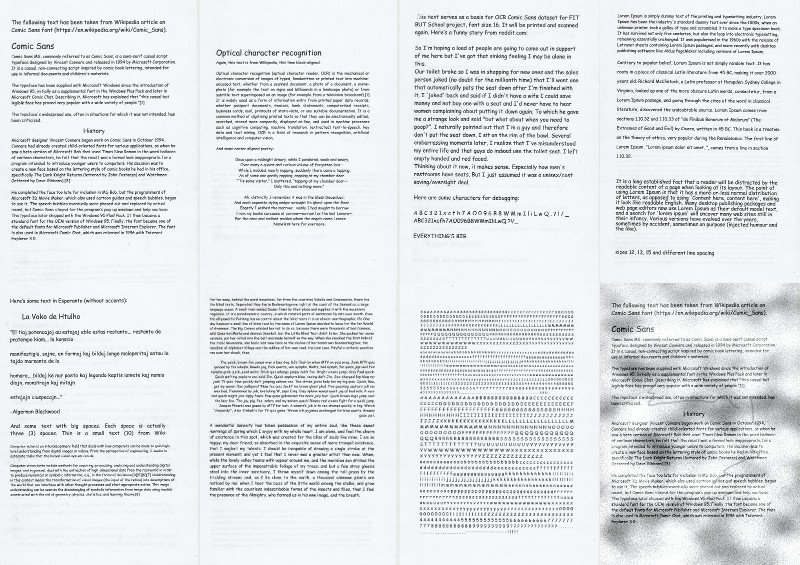
\includegraphics[width=13.5cm,keepaspectratio]{pages.jpg}
  \caption{strany 1 - 7 (zleva doprava, shora dolů) a~zašuměná strana 1}
  \label{fig:pages}
\end{figure}

\begin{figure}[htb]
  \centering
  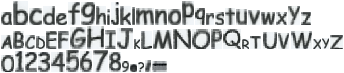
\includegraphics[width=13.5cm,keepaspectratio]{averages.png}
  \caption{průměrné obrazy vzorků}
  \label{fig:avg}
\end{figure}

\subsection{Segmentace}

Segmentace hledá nejprve řádky a~poté jednotlivé znaky v~těchto řádcích -- algoritmus je pokaždé stejný, jen
se segmentuje podél různých dimenzí. Toto provádí funkce {\tt segmentation\_1d}, která iteruje po
řádcích/sloupcích obrazu a~podle prahu průměrné intenzity vytváří spojité segmenty, které navíc nesmí být příliš malé
ani velké (malé segmenty se zahazují, velké rozdělují).

Každý nalezený výřez je ještě před klasifikací upraven tak, že se posunou jeho okraje na pokud možno přesnou hranici znaku
(pomocí funkce {\tt correct\_character\_cutout}).

Mezery se určují podle vzdálenosti segmentů (0,3 výšky řádku).

\begin{figure}[htb]
  \centering
  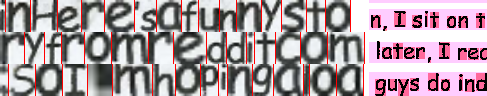
\includegraphics[width=13.5cm,keepaspectratio]{cutouts.png}
  \caption{ukázky segmentace}
\end{figure}

\subsection{Klasifikace}

Program nabízí následující klasifikátory:

\begin{itemize}
  \item rastrový klasifikátor \cite{ocr} - Velmi jednoduchý klasifikátor, který porovnává získaný výřez s~průměrným obrazem každého vzorku pomocí korelace. Bere částečně v~potaz i~poměr rozměrů vzorku a~průměrnou intenzitu.
  \item KNN, HoG příznaky - K-nearest-neighbours algoritmus na základě histogramů orientovaných gradientů.
  \item SVM, HoG příznaky - Support vector machine algoritmus na základě histogramů orientovaných gradientů.
  \item MLP - Multilayer perceptron dopředná neuronová síť. Do sítě vstupuje samotný výřez převedený do stupňů šedi a~zmenšený na velikost $10 \times 10$ pixelů. Parametry sítě jsme nalezli experimentálně: 
    \begin{itemize}
      \item vrstvy: 100, 35, 20, 1
      \item backpropagation trénování, maximum 50 iterací, $\epsilon = 10^{-9}$
    \end{itemize}
  \item složený klasifikátor - Využívá všechny výše zmíněné klasifikátory ke hlasování. Není-li při hlasování většina, bere se názor nejúspěšnějšího klasifikátoru (SVM).
\end{itemize}

Natrénované modely klasifikátorů se ukládají do XML souborů, aby trénování neprobíhalo při každém spuštění znovu.

\section{Testování}

Pro testování jsme využili vlastní skenované stránky (viz obr. \ref{fig:pages}). Metrikou
při porovnání s~referenčními přepisy byla Levenshteinova vzdálenost, tzn. počet editačních kroků. \cite{lev}
Využili jsme vlastní automatizované testy napsané v~jazycích Python a BASH.

Dále jsme porovnávali naše řešení s~kvalitním open-source OCR enginem Tesseract. \cite{tess} Tesseract
je velmi komplexní a~je postaven na spoustě pokročilých technologií (baseline fitting, slovníky, neuronové sítě,
dvouprůchodové algoritmy apod.). \cite{tess2}

Testovali jsme rovněž samotnou segmentaci tak, že jsme porovnávali výstupní a~referenční texty, v~nichž jsme
nahradili všechny znaky kromě mezer jedním stejným znakem, takže se ignorovala klasifikace.

%%%%%%%%%%%%%%%%%%%%%%%%%%%%%%%%%%%%%%%%%%%%%%%%%%%%%%%%%%%%%%%%%%%%%%%%%%%%%%%%%%%%%%%%

\section{Vyhodnocení}

Z~tabulky \ref{tab:tests} vidíme, že nejúspěšnější klasifikátor byl SVM. Jde-li o rychlost, zdaleka nejlepší
byl rastrový klasifikátor. Tesseract měl jednoznačně nejmenší chybu na běžných testech, při dobré rychlosti,
avšak kvůli slovníkovým metodám selhával na str. 5 (Esperanto bez diakritiky), 6 (místní názvy a~nestandardní
slova) a~7 (seznam znaků). Náš program měl problém se segmentací textu s~malým řádkováním
na str. 4.

\begin{table}[htb]
{\scriptsize
\begin{tabular}{|l|l|l|l|l|l|l|l|l|l|} 
  \hline
  prog. & klas. & str 1 & str 2 & str 3 & str 4 & str 5 & str 6 & str 7 & prům. \\
  \hline\hline
  POV   & segm. & 130, 0.1 & 162, 0.1 & 47, 0.1  & 720, 0.1 & 163, 0.1 & 333, 0.2 & 148, 0.1 & 243, 0.1 \\
  \hline
  POV   & rast. & 492, 0.4 & 525, 0.3 & 231, 0.3 & 969, 0.3 & 457, 0.3 & 1031, 0.5& 396, 0.4 & 585, 0.4 \\
  \hline
  POV   & KNN   & 377, 36  & 445, 32  & 163, 29  & 896, 30  & 412, 29  & 878, 54  & 247, 42  & 488, 36  \\
  \hline
  POV   & SVM   & 295, 26  & 378, 24  & 114, 22  & 859, 23  & 356, 23  & 757, 30  & 176, 27  & 419, 25  \\
  \hline
  POV   & MLP   & 1504, 3  & 1381, 3  & 917, 3   & 1545, 3  & 1108, 3  & 2405, 3  & 1776, 3  & 1519, 3  \\
  \hline
  POV   & komb  & 309, 46  & 378, 43  & 124, 36  & 865, 36  & 359, 49  & 753, 61  & 186, 53  & 424, 45  \\
  \hline
  Tess  & segm. & 68, 10   & 167, 13  & 64, 3    & 67, 8    & 387, 13  & 279, 32  & 2383, 7  & 487, 12  \\
  \hline
\end{tabular}
}
\caption{Výsledky testů na zmenšených skenech ve formátu [chyba (Levenshteinova vzdálenost), čas v~s]. Časy zahrnují dobu trénování. Průměrný počet znaků na stranu je 2285.}
\label{tab:tests}
\end{table}

\begin{table}[htb]
{\scriptsize
\begin{tabular}{ |l|l|l|l| } 
  \hline
  program, klasifikátor & sken                 & čas (s) & chyba \\
  \hline\hline
  Tesseract             & page 1 (orig. rezl.) & 4       & 26    \\
  \hline
  POV, SVM              & page 1 (orig. rezl.) & 27      & 177   \\
  \hline
  Tesseract             & page 2 (orig. rezl.) & 4       & 164   \\
  \hline
  POV, SVM              & page 2 (orig. rezl.) & 26      & 195   \\
  \hline
  Tesseract             & page 1 small noise   & 2       & 2003  \\
  \hline
  POV, SVM              & page 1 small noise   & 19      & 2123  \\
  \hline
  Tesseract             & page 1 noise         & 3       & 2123  \\
  \hline
  POV,SVM               & page 1 noise         & 19      & 2123  \\
  \hline
\end{tabular}
}
\caption{dodatečné testy}
\end{table}

Pro představu čitelnosti prezentujeme ukázku přepisu naším programem pomocí SVM klasifikátoru:

{
\centering
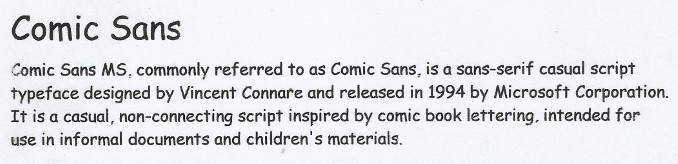
\includegraphics[width=14cm,keepaspectratio]{example.jpg}
}

{\tt\footnotesize ~\\
Comic Sans\\
Comic Sans MS commonly referred to as Comic Sans- is a sans serif casual scri,\\
lptace designed by Vincem -nnar and released in 1994 by Microsoft CorpoHtion\\
It is a c-ual- noTconmcti- script inspirl by comic book lJteriM imended for\\
use in informal documems and children-s mterials
}

%%%%%%%%%%%%%%%%%%%%%%%%%%%%%%%%%%%%%%%%%%%%%%%%%%%%%%%%%%%%%%%%%%%%%%%%%%%%%%%%%%%%%%%%

\section{Závěr}

Implementovali jsme OCR systém pro font Comic Sans a~vyhodnotili jeho aspekty. Ty jsme porovnali s~používaným systémem Tesseract. Mezi hlavní zjištěné závěry patří:

\begin{itemize}
  \item Při dobré kvalitě skenů je jednoduchý přístup velmi použitelný i~na obecný text, texty jsou více či méně čitelné. Tesseract je stále mnohem kvalitnější,
        robustnější a~obecnější, avšak někdy i~pomalejší a~horší při použití nestandardních jazyků.
  \item Spíše než dále zlepšovat klasifikátory by pravděpodobně bylo lepší zavést slovníky.
  \item Zmenšujeme-li výřez znaku na minimální možnou velikost, máme problém s~rozlišování znaků jako ",.'".
  \item Bylo by lepší použít konvoluční neuronovou síť než MLP.
  \item Náš způsob segmentace selhává při malém řádkování.
\end{itemize}

\bibliographystyle{abbrv}
\begin{flushleft}
  \bibliography{project}
\end{flushleft}

%\appendix
%\newpage
%\section{}

\end{document}
